\ifgerman{\chapter{Auswertung}}{\chapter{Implementation}}
\label{sec:implementation}

\section{Simulation Environment}

The FINken consists of the body, the rotors and the sensors. The body contains the behavioural and flight control, the thrust simulation is handled by scripts connected to the rotor structure.

\subsection{Scene Modeling}

The body consists of multiple objects, while visual representation and the physical behaviour are split. For visual representation, a *.stl file from the CAD-Model of the original FINken was imported. This shape is rather complex, which makes the simulation time consuming. To speed up the simulation, the shape of the finken was remodelled in VREP, using only simple rectangular shapes. Making the complex shape static, establishing a fixed connection and hiding the simple shape, the result is a a visual appealing simulation object with good simulation performance. A dummy-object is used as a singular measurement reference point in the middle of the FINken. This has to be taken into account when targeting physical objects, as the FINken will not be able to reach the target completely without colliding with the object. This dummy object should always be used when refering to the FINkens position, orientation or movements, as it is aligned to the global coordinate system while especially imported shapes may be rotated in the simulation. Vrep provides several pre-configured sensor type, the real FINkens sensors were modeled by using existing ultrasound distance sensors. The FINken is equipped with Maxbotix MB1232: I2CXL-MaxSonar-EZ3 sensors\url{(http://www.maxbotix.com/documents/I2CXL-MaxSonar-EZ_Datasheet.pdf}). According to the datasheet, they have an opening angle of $\angle{30}$ at maximum range when detecting smaller objects and maximum range of 7.65m for larger objects as walls. The datasheet states a rather complex beam shape, but for the simulation a cone with an opening angle of $\angle{30}$  and a height of 7.65m will be used. Finally, a dummy target objects belongs the virtual FINken. This object can be moved manually in the scene and the simulated quadcopter will fly towards it.  As the real FINken doesn't have the ability to fly to predefined points, we only used this feature for development.

\begin{figure}[h!]
 \begin{center}
  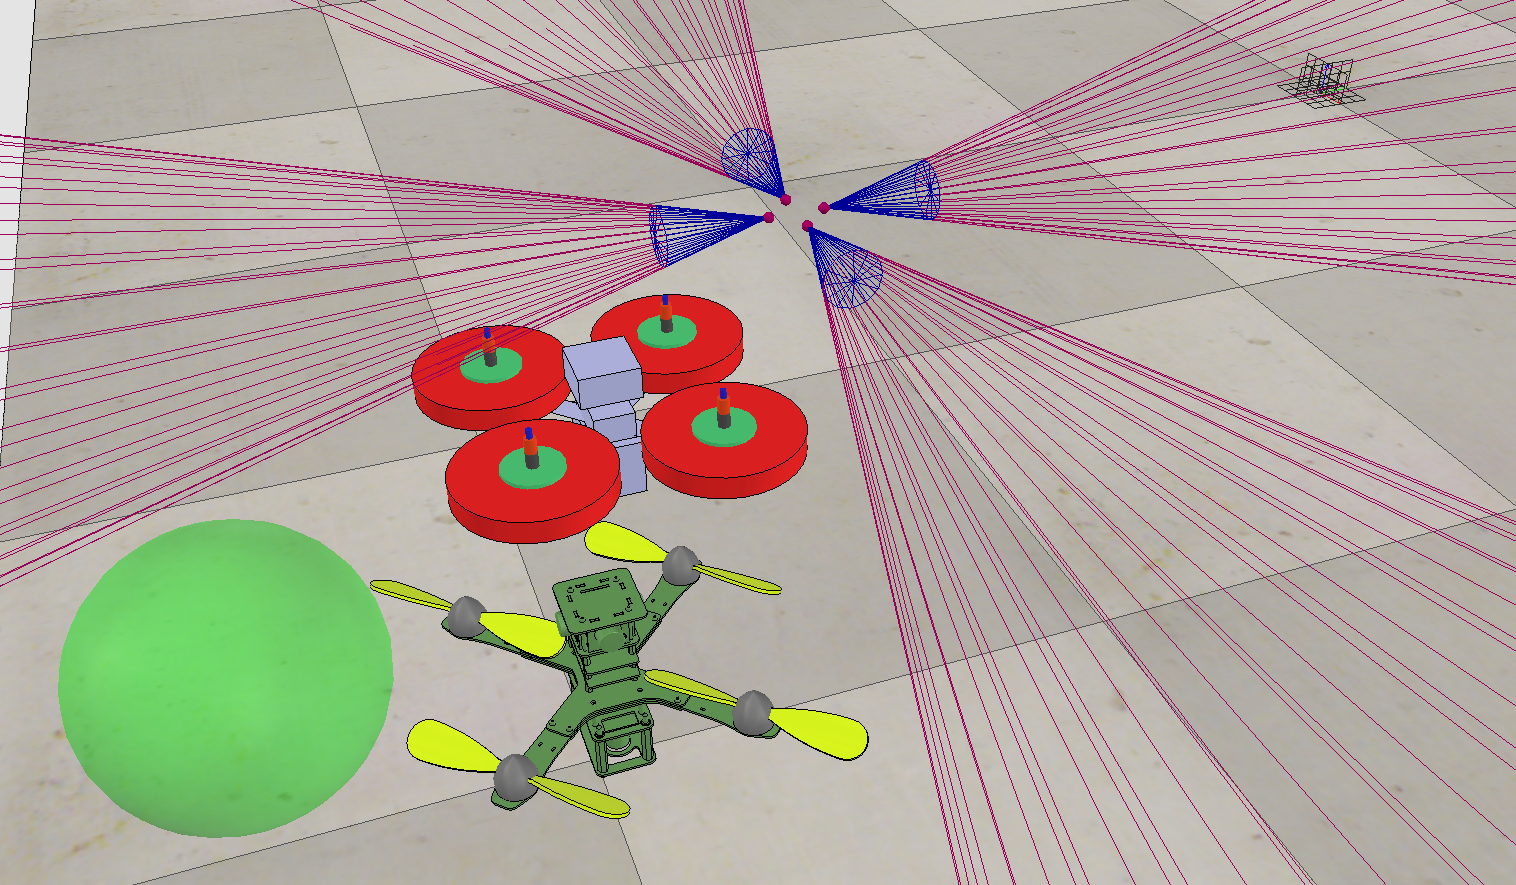
\includegraphics[width=\linewidth]{vrepDisassemlbyFull.png}
 \end{center}
  \caption{Parts of the simulation object \label{fig:vrepParts}}
\end{figure}

The measured weight of the real FINken was applied to the simulation object. As no advanced modelling like calculating moments of inertia was done, the weight of the motor was applied separately to the rotor model in VREP.  The motor assembly adds significant weight outside the FINkens center of gravity and therefore has a rather large influence on its behaviour. 
\todo{weight table for finken2 and finken3}
The linear damping factor of the FINken body material was set to 0.3, to decrease drift and to model the air resistance of the real FINken, which is minimal but nevertheless existent.


The rotor model in VREP handles the thrust simulation and thus a huge part of the physical behaviour of the quadcopter model.  Again, visual representation and physical simulation are separated. 
\todo{add picture of rotor}
The visualisation is done with a static shape of a rotor, that is connected to a joint and rotates with a fixed speed. During flight, the rotation speed does not really change visually noticeable, a dynamic adaption of the rotation would only increase computation time without much benefit. Of course, the rotor shape could be made non-static and rotate in a particle stream, and apply the thrust force according to the particle collisions, but again, this would mean a massive increase of computation power and is not needed for our purposes.

\begin{figure}[h!]
 \begin{center}
  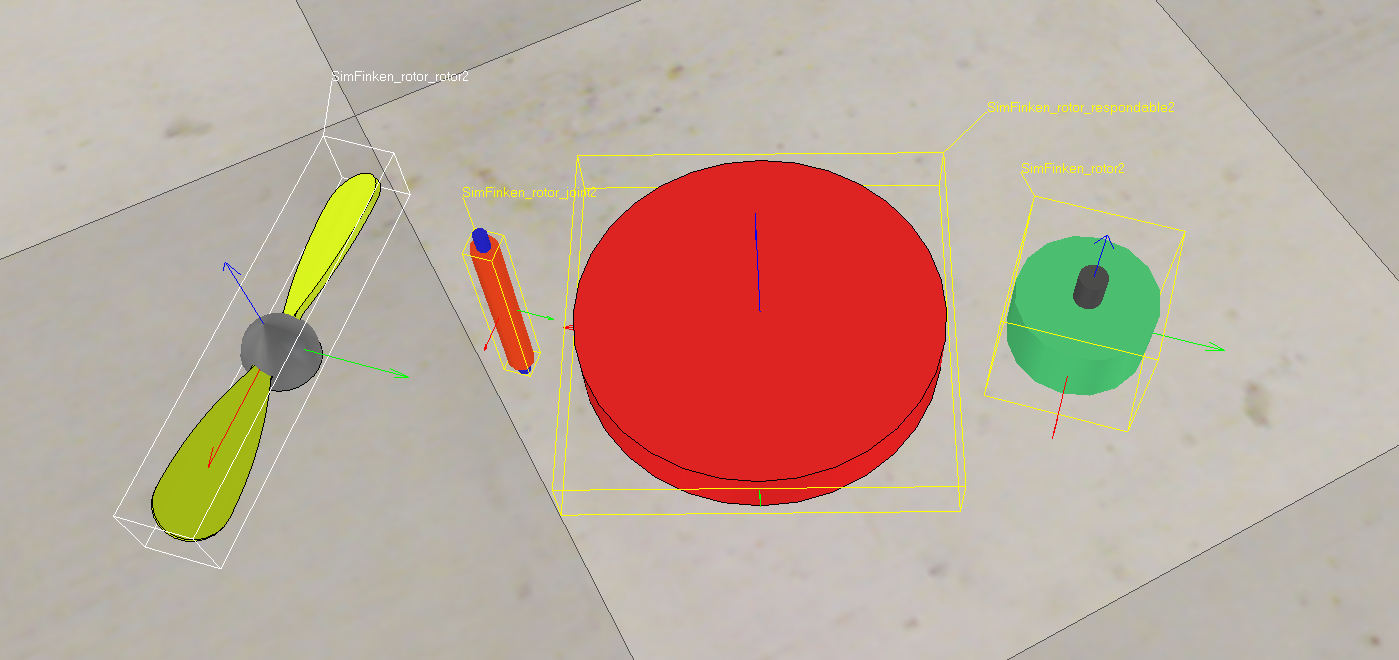
\includegraphics[width=\linewidth]{vrepRotorLegend}
 \end{center}
  \caption{Parts of the simulated rotor \label{fig:vrepRotor}}
\end{figure}


The rotor model is attached to the FINken body via a force sensor which applies the forces and torques calculated in the physical rotor model to the FINken body. The rotor is represented by a cylindrical shape which resembles the area swept by a real rotor and uses a particle simulation to emulate the airstream. The handling of the particle simulation is done inside a lua child script attached to the rotor model. The script has several parameters for the particle simulation, \todo{add complete param list}.
During simulation, the particle velocity is the parameter used to control the finken. This rotor model was already included in VREP as an example and was used without further modifications, the theory behind it is shortly explained in \ref{sec:theomodel}. Using the particle simulation has the advantage of providing a small random factor that causes noise and it simulates the airstream which will influence  other copters in multicopter scenarios.



\subsection{Flight controller in simulation}

The V-REP example quadrocopter already included some flight controller out of the box

\begin{itemize}
\item{PID implementation with I-reset}
\item{}
\item{}
\item{}
\end{itemize}
\todo{finken parameter estimation}

\todo{controller tuning}


\begin{table}[h]
	\centering
	\begin{tabular}{|c|c|}
    		\hline
		Parameter & Value \\
		\hline
    		Physics engine & Bullet\\
    		\hline
    		Dynamics settings & Accurate (default) \\
    		\hline
    		Simulation time step & 50 ms (default) \\
    		\hline
    		Real-time mode & enabled \\
    		\hline
	\end{tabular}
    	\caption{V-REP simulation parameters}
      	\label{tab:simSettings}
\end{table}

\subsection{Simulation Software Structure}

\todo{finish diagram of finken software}
\tikzset{
    group/.style={
           rectangle,
           rounded corners,
           draw=black, very thick,
           minimum height=2em,
           inner sep=2pt,
           text centered,
           },
           swScript/.style={
           rectangle,
           draw=black, very thick,
           minimum height=2em,
           inner sep=2pt,
           align = left,
           },
           vrepObject/.style={
           circle,
           draw=black, very thick,
           minimum height=2em,
           inner sep=2pt,
           text centered,
           },
           vrepEnv/.style={
           ellipse,
           draw=black, very thick,
           minimum height = 5cm,
           minimum width = 3cm,
           },
            implements/.style={
            -{open triangle 60}, dashed
           },
           inherits/.style={
           -{open triangle 60},
           }
}
\begin{figure}[h]
	\centering
	\begin{tikzpicture}[scale=2, node distance = 1cm, auto]
		%vrep part
		\node[vrepEnv](vrep){};
		\node[below=0.3cm of vrep.north]{\underline{V-REP}};
		\node[vrepObject, below =1.1cm of vrep.north](fink1){finken1};
		\node[vrepObject, below =0.4cm of fink1.south](fink2){finken2};
		%lua script part
		\node[swScript, rectangle split, rectangle split,rectangle split parts=3, right=of vrep.45](finkenMeta){finkenMeta\nodepart{second}
			public:
			\nodepart{third}
			public: \\
			step() \\
			sense() };
		\node[swScript, rectangle split, rectangle split,rectangle split parts=3, below=of finkenMeta](finken){finken\nodepart{second}
			public:
			\nodepart{third}
			public: \\
			step() \\
			sense() };
		\node[swScript][rectangle split, rectangle split,rectangle split parts=3, right=of finken](finkenCore){finkenCore 
			\nodepart{second}
			public:
			\nodepart{third}
			public: \\
			step() \\
			sense()}; 
		\node[swScript, rectangle split, rectangle split,rectangle split parts=3, above=of finkenCore](finkenPID){finkenPID\nodepart{second}
			public:
			\nodepart{third}
			public: \\
			init(P,I,D) \\
			step(error, $\delta$t) };
		%connections
		\draw[inherits] (finken) to (finkenCore); 
		\draw[-{angle 60}](finkenCore) to (finkenPID);
		\draw[implements](fink1) to (finken);
		\draw[implements](fink2) to (finken) ;
		\draw[implements](vrep.45) to (finkenMeta);
	\end{tikzpicture}
	\caption{Software structure of the FINken Simulation}
	\label{fig:finkenSoftStruct}
\end{figure}

The simulation software is written in Lua and runs inside a non-threaded child script of each FINken quadrocopter in VREP.  

The base class is the finkenCore, which contains the main flight control algorithm and a steering interface as well as an interface to the FINkens sensors.
The input commands for controlling the FINken are set via the signal communication of VREP. Signals inside VREP are the most versatile communication possibility which can be accessed from anywhere inside VREP and any remote API, they can be seen as a kind of global variable. Signals can be of integer, float or string type, where custom data types can be sent in text form as string signals. 

The finkenCore needs to be initialized at simulation start the for each simulated FINken. It starts the VREP remote API server and creates the API signals. Also, the PID controllers for flight control are initialized. 
During simulation, calling the FINkenCore.step() method handles the flight control. The input values are read from the signals \textit{pitch}, \textit{roll}, \textit{yaw} and \textit{throttle}. When the signal \textit{height} has a positive value, the FINkenCore will control the thrust so that the simulated FINken will keep the height provided by the signal, otherweise only the \textit{throttle} signal is used directly. The previously initialized PID controllers are used to compute the target air stream velocity for each rotor to move the simulated FINken to the target orientation.

To keep a quadcopter at a certain height without an external reference requires an exact equilibrium between gravity and thrust. The current real FINkens do not compensate the battery voltage, so the same throttle corresponds to different thrust forces during flight. Also, each FINken unit has slightly different base thrust. Therefore, the thrust in the simulation is tuned with a logisitc curve \ref{equ:logistic} to decrease the influence of the throttle close to the hover thrust. 
\begin{equation}
throttle_{tuned} = \begin{cases}
-\frac{a * |throttle|}{a - |throttle| + 50} + 50 & throttle < 0 \\
\frac{b * throttle}{b - throttle + 50} + 50 & throttle >= 0\\
\end{cases}
\label{equ:logistic}
\end{equation}
The default values for the throttle tuning function are  $a = 1$ and $b = 1$. 
\todo{insert plot of function?}


The simulated FINken is equipped with 4 distance sensors which resemble the 4 ultrasound sensors of the real FINken. The FINkenCore module contains a \textit{sense()} function that reads the 4 distance sensors and writes the values to the signal \textit{sensor\_dist}. As signals only support limited data types, \textit{sensor\_dist} is a string signal containing a packed float array. The array contains the distances in the order \textit{front}, \textit{left}, \textit{back}, \textit{right}.  If the FINken gets more sensors in the future, their evaluation has to be added to this method.
By writing the distance values to a signal, they can be propagated to the Ivy-Bus and thus to the real FINken by our Java communication app, which enables the real FINken to detect virtual objects, as simulated FINken or walls that only exist in the Simulation.


While the FINken is normally controlled by setting the pitch, roll, yaw and throttle directly, an alternative is to specify a target object. This method was originally used by the example quadcopter model of V-REP, though the function works differently in the FINkenCore now. When calling  \textit{setTarget(targetObject)}, the differences in x, y and z coordinates of the FINken base to the target objects are given to three PID controllers which calculate the pitch, roll and throttle to move the FINken to the target objects position. Those values are then published via the control signals for the FINken and regularly processed by it's internal controls. Therefore, \textit{setTarget(tragetObject)} needs to be called every time before \textit{step()}, when a target object should be approached.

In the previous sections, only the signal names for the first simulated FINken were used for better readability. As the simulation is scalable, more than one FINken can be added, therefore a naming scheme for signals is needed to prevent collisions of the globally visible signals. The signals corresponding to the first FINken are \textit{pitch}, \textit{roll}, \textit{yaw}, \textit{throttle}, \textit{height} and \textit{sensor\_dist}. For the second FINken, when the first one is copied, VREP automatically adds "\#0" to it's name. Following this convention, but leaving the '\#' to prevent problems with special characters when forwarding the signals through our interface, we add '0' to the signal names for the second FINken and consecutively enumerate following FINkens.

The finken.lua module provides an basic structure for further enhancements. It's contained functions like \textit{step()} and \textit{sense()} are called called inside V-REP during the appropriate simulation step sections. By calling custom functions inside those functions, the behaviour of the FINkens can be customised without any need to change the lua scripts inside V-REP. If a heterogenous swarm of FINkens with different functionalities should be implemented, the different finken-scripts have to be imported by the different FINkens in the simulation, which needs to be done in the lua scripts inside V-REP.


FinkenMeta.lua is loaded in the child script of a dummy object in the scene  to have an API to the simulation that is not connected to a single FINken. This can be used to dynamically manipulate the environment during simulation, e.g. by adding objects like other FINkens.
\section{Communication V-REP - Quadrocopters}
\label{sec:commImplementation}

This chapter describes the implementation of the requirements on the Java-API, which ware discussed in \ref{sec:communication} of \ref{chap:theo}. It begins with an overview of the software architecture and continues with the explanation of the created projects, classes and their use. It helps understanding how the communication between the V-REP and the quadrocopters is implemented and how to use the API or extend it in order to implement other mixed-reality scenarios.\\
Note that this is just a brief explanation of the Java-API implementation. If you want to go in details refer to the Javadoc which is also provided as an attachment to this paper.

\subsection{Software architecture}

The software architecture of the Java-API, which serves as a communication bridge between the Paparazzi software and the V-REP simulation, is designed to be as modular as possible in order to facilitate the further development of the project. Its reusable components should also serve as a building blocks for the students that want to develop future mixed-reality projects. \\

On \ref{fig:apiArchitecture} is depicted an raw overview of the Java-API software architecture.
The final program is assembled from independently developed components. Each part is independent and provide well-defined exported interfaces so that the other parts can use them.
The first layer contains the projects \textit{JavaV-REP}, \textit{JavaIvyBus} and \textit{JavaXmlSax}.\\
The \textit{JavaV-REP} is the implementation of the requirements concerning V-REP, that ware discussed in \ref{sec:requirementsVREP} of \ref{chap:theo}. At the heart of this project is the V-REP Remote-API binding for Java provided by Coppelia. The \textit{JavaVrep} project extends this library and provides further utility methods for establishing connection to remote V-REP servers as well as retrieving and manipulating scene objects. The \textit{JavaV-REP} project is described in more details in \ref{sec:vrepImplementation}.\\

\begin{figure}[h!]
 \begin{center}
  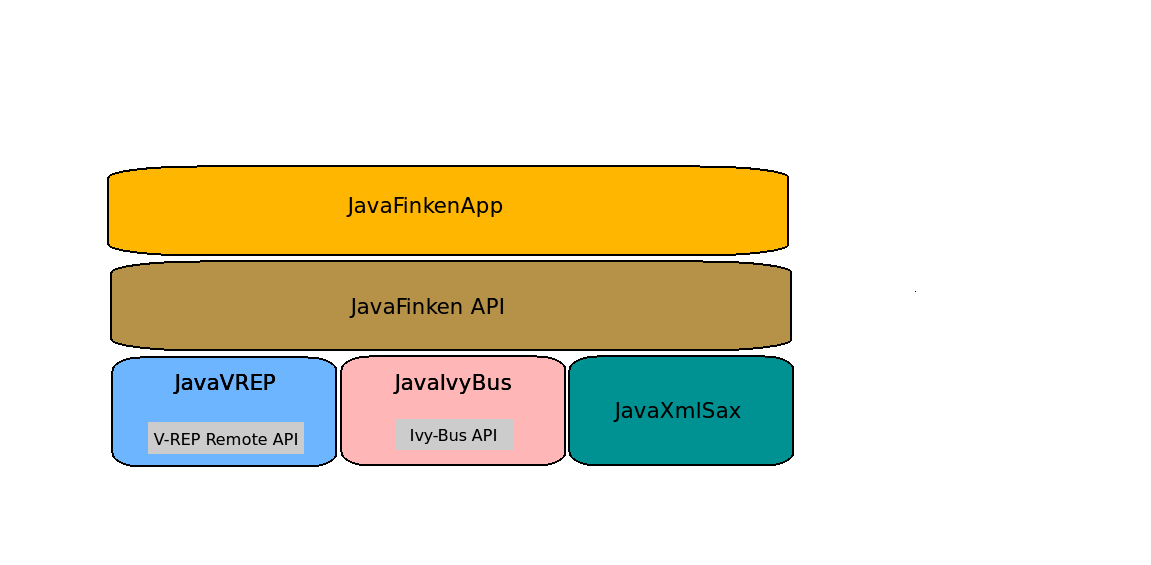
\includegraphics[scale=0.6]{apiArchitecture.png}
 \end{center}
  \caption{Java-API architecture\label{fig:apiArchitecture}}
\end{figure}

\textit{JavaIvyBus} is a Java project, that imports the Ivy-Bus library and implements the requirements regarding Ivy-Bus, which ware discussed in \ref{sec:requirementsIVYBus}.\\ 
It extends the functionality of the the Ivy-Bus library and provides the programmer with the possibility to create Ivy-Bus nodes by just instantiating an object which takes as constructor parameter the name of the bus-node. It facilitates the connection or disconnection from the bus by just calling a function the the created bus-node object. The abstractions on which this project rely also allow to easily create bus messages or just parse them from xml file and subscribe to them even dynamically. The \textit{JavaIvyBus} project is discussed in more detail in \ref{sec:ivyBusImplementation}. \\

The \textit{JavaXmlSax} project is a small API, that allows the programmer to easily create a custom xml reader that parses any xml document and retrieves the instances of the objects defined by the xml. It consists of several abstract classes, that provide the template for the custom xml readers.\\
A short explanation of how this API can be used is included in \ref{sec:xmlImplementation}. \\

On the next layer in the hierarchy is the \textit{JavaFinken} API. It uses the APIs from the layer below to provide further abstractions and utilities for our FINKEN project. It consists of classes that describe 
the aircrafts defined in the paparazzi, defines the basic classes that represent our virtual and real quadrocopters and their sensors, defines a representation of the telemetry and the V-REP signals. With the help of \textit{JavaIvyBus} API, lying on the layer below, the Ivy-Bus nodes, specific for the virtual and real quadrocopters are represented. The abstraction provided by \textit{JavaXmlSax} is used to create a custom Xml readers for parsing the telemetry, messages and aircrafts from the Xml files. A more detailed description of the API is included in \ref{sec:javaFinkenImplementation} \\

On the top of the hierarchy is situated the actual application of our project called \textit{JavaFinkenAPP}. It uses \textit{JavaFinken} API to bind the provided utility classes in a specific application meeting our project requirements. The application has a simple Graphical User Interface that facilitates specifying the IP and Port number of the V-REP simulation server, specifying path to the paparazzi software, a button for establishing the connection and other UI elements.




\subsection{JavaV-REP}
\label{sec:vrepImplementation}

All the functionality, that concerns V-REP and was discussed in \ref{sec:requirementsVREP} of \ref{chap:theo} is implemented as a single Java project called \textit{JavaVREP}.\\
 The project uses the V-REP Remote-API Java binding - package \textit{coppelia} (containing 12 Java classes) and the \textit{libremoteApiJava.so} or \textit{libremoteApiJava.dll} (depending if the platform is Linux or Windows). The \textit{libremoteApiJava.so} should be placed in the Java home directory, e.g \textit{/usr/lib/jvm/java-8-oracle/jre/lib/amd64}, in order for the project to be compiled.\\
The main class is the \textit{VrepConnection.java}, which is a wrapper of the \textit{remoteApi.java} class provided by the V-REP remote API. Its singleton instance can be retrieved by calling:

\begin{center}
\begin{tabular}{c}
\begin{lstlisting}[basicstyle=\small]
VrepConnection connection = VrepConnectionUtils.getConnection();
\end{lstlisting}
\end{tabular}
\end{center}

The above expression loads the remote API library and returns the instance of \textit{VrepConnection} on which the Remote API functions are called. For example to retrieve all objects in a scene the following function have to be called on the \textit{VrepConnection} instance:

\begin{center}
\begin{tabular}{c}
\begin{lstlisting}[basicstyle=\small]

connection.simxGetObjects();

\end{lstlisting}
\end{tabular}
\end{center}

The interfaces \textit{VrepServer} and \textit{VrepClient} and their implementations \textit{StandardVrepServer} and \textit{StandardVrepClient} describe the two end-points of the communication. The \textit{VrepServer} describes the IP address and the port number of the machine on which the V-REP is running. In order to connect to a V-REP server we have to create in instance of the \textit{VrepServer} and open the client:

\begin{center}
\begin{tabular}{c}
\begin{lstlisting}[basicstyle=\small, language=Java]
VrepConnection connection;
VrepClient     client;
VrepServer     server;

connection = VrepConnectionUtils.getConnection();
client     = VrepClientUtils.getClient();
server     = new StandardVrepServer("127.0.0.1", "19999");

client.connectToServer(server);

if (!client.isConnected()) {
// error in connection
} 
\end{lstlisting}
\end{tabular}
\end{center}

The above example shows how to connect to a V-REP server. The IP \textit{127.0.0.1} specifies that the server is running on the same machine. The port number can be chosen arbitrary, but have to match on both client and server site.\\
In order to close the connection just the method \textit{client.close()} has to be called. \\

The \textit{VrepClient} conforms to the Java Beans specification and can thus fire events when the connection has been established or disconnected. Any class who is interested in catching these events asynchronously, for example GUI, will have to implement \textit{PropertyChangeListener} and register. See
\url{https://docs.oracle.com/javase/tutorial/javabeans/writing/events.html} for more information. \\

Each V-REP scene object is represented by the interface \textit{VrepObject} and the \textit{AbsVrepObject} represents an abstract scene object from which all types of object derive. The abstract scene object has private properties like \textit{Position}, \textit{Orientation}, \textit{LinearVelocity} and \textit{AngularVelocity}, which represent its inertial parameters taken from the V-REP.
\textit{VrepObjectType} is an Enum, that specifies the scene object type like Shape, Path, Proximity sensor etc. The name of the scene object is represented by the class \textit{VrepObjectName}, which consists of a base name and an index. If an object is copy-pasted (multiple instances of an object), then
each instance of the object receives the following name, according to V-REP naming scheme: \textit{\texttt{base\_name\#index}}. For example if we want to have three quadrocopters, their names in V-REP will be represented as follows: \textit{\texttt{Quad\_Lia\_ovgu\_01}}, \textit{\texttt{Quad\_Lia\_ovgu\_02\#0}} and \textit{\texttt{Quad\_Lia\_ovgu\_03\#1}}. \\

The V-REP scene is represented by the class \textit{VrepScene}, which retrieves all objects and hold a collection of them for further use. Since we always have one V-REP scene the class is designed as a Singleton pattern. The following example shows how this class is used for loading the scene and retrieving all shape objects.

\begin{center}
\begin{tabular}{c}
\begin{lstlisting}[basicstyle=\small, language=Java]
VrepScene   scene;
List<Shape> shapeObjects;

scene = VrepSceneUtils.getVrepScene();
scene.loadScene();
shapeObjects = scene.getAllShapeObjects();

\end{lstlisting}
\end{tabular}
\end{center}

The project \textit{JavaVrep} also defines the interface \textit{ObjectUpdator} and its abstract implementation \textit{AbsObjectUpdator}, which is used to update the \textit{VrepObject}s with real-time parameters from V-REP, like their \textit{Position}, \textit{Orientation}, \textit{LinearVelocity} and \textit{AngularVelovity}.


\subsection{JavaIvyBus}
\label{sec:ivyBusImplementation}

The requirements regarding the Ivy-Bus, that ware stated in \ref{sec:requirementsIVYBus} of \ref{chap:theo} are implemented in a stand-alone Java project called \textit{JavaIvyBus}. \\
The project requires the \textit{ivy-java.jar} library to be on its class path in order to be compiled.\\
The project contains class definitions of the Paparazzi messages that are defined in a Xml file. See listing \ref{lst:MessageXml} of \ref{chap:theo}. The interface \textit{Message} and its abstract implementation \textit{AbsMessage} describe such a message with its name, period at which the message is sent, identifier and \textit{MessageField}s. \\
The interface \textit{IvyBusNode} represents a single independent node communicating on the common bus. By inheriting from its abstract implementation \textit{AbsIvyBusNode}, one can create a custom bus-node. The methods \textit{IvyBusNode.connect()} and \textit{IvyBusNode.disconnect()} are used to attach the particular node to the bus and disconnect it. The \textit{IvyBusNode} also conforms to the Java Beans specification and and fires asynchronous notifications each time the node joins or leaves the bus.
After obtaining an instance of a \textit{Message}, parsed from the Xml file or a custom-created, the bus-node can subscribe to this \textit{Message} by invoking the method \textit{IvyBusNode.subscribeToMessage(Message msg)} and thus receive all the messages of this kind or use the method \textit{IvyBusNode.subscribeToIdMessage(Message msg, int id)}, which subscribes to the messages published just by this quadrocopter ehich has the same id. \\
Once a \textit{Message} to which the bus node has subscribed has been received, the bus node fires an notification and gives the instance of the received \textit{Message}, with all of its \textit{MessageField}s initialized with the actual message values. The following listing shows an example hot to subscribe to a message and get asynchronous notification when the message is received.

\begin{center}
\begin{tabular}{c}
\begin{lstlisting}[basicstyle=\small, language=Java]

class TestBusNode implements PropertyChangeListener {
  
  private IvyBusNode node; 
  private Message    message;
  
  public TestBusNode(IvyBusNode node, Message msg) {
    this.node    = node;
    this.message = msg;
    
    this.node.addPropertyChangeListener(this);
    this.node.subscribeToMessage(this.message);
  }
  
  @override
  public void propertyChange(PropertyChangeEvent event) {
    Message receivedMessage;
    
    // the message has been received
        
    receivedMessage = (Message)event.getNewValue();    
  }

}

\end{lstlisting}
\end{tabular}
\end{center}


\subsection{JavaXmlSax}
\label{sec:xmlImplementation}

The project \textit{JavaXmlSax} was created with the idea in mind to provide a small, modular API, that gives the developer an abstract building block for fast and easy development of custom XML file readers. It uses the \href{http://www.saxproject.org/}{SAX Java API} and extends it in order to provide a template for fast creation of specific XML readers.\\
The basic class in this module is the abstract class \textit{AbsSaxXmlReader}. It encapsulates all necessary classes needed for creating and handling of the XML parsing and defines abstract methods, which allow its subclasses to provide their specific parsing criteria. Thus the developer can concentrate on the actual parsing logic and don't have to take care of setting up and managing the necessary input streams and files.\

To create a specific XML reader we have to create a class, which extends the \textit{AbsXmlReader} and provides implementation of the abstract methods \textit{onStartElementRead} and \textit{onStopElementRead}.These methods are called when the \textit{AbsSaxXmlReader} encounters start or end XML tag. It is the role of the subclass to fetch the necessary attributes and create an instance of the XML element, when \textit{onStartElementRead} is called and store the instance in some sort of collection, when the closing tag of the element is reached. \
The code below shows an example of how the XML parser can be used.

\begin{center}
\begin{tabular}{c}
\begin{lstlisting}[basicstyle=\small, language=Java]

MessageXmlReader msgReader;
List<Message>    messages;

msgReader = new MessageXmlReader("/home/paparazzi/conf/messages.xml");

msgReader.parseXmlDocument();

messages  = msgReader.getMessages();

\end{lstlisting}
\end{tabular}
\end{center}


\subsection{JavaFinken}
\label{sec:javaFinkenImplementation}

The \textit{JavaFinken} API is a project that relies on the previously introduced projects \textit{JavaV-REP}, \textit{JavaIvyBus} and \textit{JavaXmlSax}. It represents the implementation of the application requirements introduced in \ref{sec:requirementsApplication} and provides the basic classes and utilities upon which our application can be built.\\

The class of a special importance is the \textit{AbsFinkenDrone}, which represents the abstract quadrocopter and is described by the interface \textit{FinkenDrone}, which on itself extends the \textit{VrepObject} interface.\\
The virtual and real quadrocopters are represented by the classes \textit{StandardRealFinkenDrone} and \textit{StandardVirtualFinkenDrone}, which extend the abstract \textit{AbsFinkenDrone}.\\
The class \textit{FinkenDroneScanner} is used to retrieve the instances of the quadrocopters and can be used as follows:

\begin{center}
\begin{tabular}{c}
\begin{lstlisting}[basicstyle=\small, language=Java]

List<StandardRealFinkenDrone>    realDrones;
List<StandardVirtualFinkenDrone> virtualDrones;
FinkenDroneScanner               droneScanner;

droneScanner  = new FinkenDroneScanner();
realDrones    = droneScanner.retrieveRealDrones(this.scene, this.client);
virtualDrones = droneScanner.retrieveVirtualDrones(this.scene, this.client);

\end{lstlisting}
\end{tabular}
\end{center}

\section{Quadcopter}

This project was about to build a mixed reality simulation around the FINken quadcopter, so there weren't made many changes to the quadcopter and the firmare itself. A few changes were needed, regarding calibration, the message link and the communication from VREP to the FINken. At the start of the project, the FINken II was used, but when the FINken III was released, it could directly be use as all our needed functions were compatible. In fact, the new telemetry link of the FINken III made a much faster communication possible, which helped some delay issues with V-REP as put in \ref{sec:messLink}
\subsection{FINken calibration}
\begin{itemize}
\item{The FINken has no external positioning system like GPS, so internal sensor errors will heavily affect the FINkens flight movements}
\item{During the first experiments, a strong drift could be obeserved}
\item{this drift could be traced back to an offset of the IMU of the copter }
\item{The paparazzi software already provides functionalities to calibrate sensor \todo{find and link website}}
\item{After calibration, the aircraft still moves due to noise, but the strong drifts could be eliminated}
\todo{add calibrated values?}
\end{itemize}
\subsection{FINken message link}
\label{sec:messLink}
\begin{itemize}
\item{FINkenII: Bluetooth Link, max. message frequency?}
\item{The Bluetooth Link limited the datarate, so getting new INS-Data from the real FINken for each simulation step was not possible}
\item{FINkenIII: 802.15.4 based communication}
\item{New communication allows messages to be sent every 21ms}
\item{VREP simulation runs with 50ms}
\item{even if packets are dropped, in general there is always new data for each simulation step}
\end{itemize}
\subsection{VREP to FINken communication}
\begin{itemize}
\item{to make virtual objects visible to the real FINken, they need to be send somehow from the virtual scene to the real hardware}
\item{FINken only perceives with ultrasound sensors}
\item{only the distances to virtual objects detected by the virtual FINken need to be sent}
\item{paparazzi allows to send messages via the telemetry link}
\item{in the FINkens firmware, when the distance values for the real ultrasound sensors are checked, the message with the virtual distances needs to be evaluated}
\item{because right now only collision avoidance is interesting, the minimum of the two values is used as the final distance}
\item{\todo{look at sensorModel code and add more details}}
\end{itemize}
% example for bar plots
%\begin{tikzpicture}
%  \centering
%  \begin{axis}[
%        ybar = 0,
%    height=6cm,
%    width=15cm,
%    enlarge x limits={rel=0.1},
%    axis lines*=left,
%    ymin=0,
%    ymax=50,
%     legend style={at={(0.5,-0.27)},
%        anchor=north,legend columns=-1},
%        ylabel={\#Anzahl Blöcke},
%        xlabel={Halstead Volumen},
%        cycle list = {black,black!70,black!40,black!10},
%        symbolic x coords={10,20,30,40,50,70,90,120,300,750,>750},
%     xtick=data,
%        nodes near coords,
%    every node near coord/.append style={
%        anchor=mid west,
%        rotate=90 }]
%     \addplot+[] coordinates {(10,3) (20,18) (30,8)(40,1)(50,0)(70,6)(90,6)(120,0)(300,2)(750,0)(>750,0)};
%    \addplot+[fill,text=black] coordinates {(10,3) (20,28) (30,22)(40,7)(50,2)(70,4)(90,11)(120,1)(300,1)(750,2)(>750,0)};
%   \addplot+[fill,,text=black] coordinates {(10,1) (20,1) (30,17)(40,30)(50,10)(70,17)(90,10)(120,8)(300,5)(750,1)(>750,0)};
%    \legend{Modell1,Modell2,Modell3}
%  \end{axis}
%\end{tikzpicture}
%
%
%
%\begin{tikzpicture}
%  \centering
%  \begin{axis}[
%        ybar = 0,
%    height=6cm,
%    width=15cm,
%    enlarge x limits={rel=0.1},
%    axis lines*=left,
%    ymin=0,
%    ymax=70,
%     legend style={at={(0.5,-0.27)},
%        anchor=north,legend columns=-1},
%        ylabel={\#Anzahl Blöcke},
%        xlabel={Anzahl Elemente pro Block},
%        cycle list = {black,black!70,black!40,black!10},
%        symbolic x coords={10,20,30,40,50,70,90,120,300,750,>750},
%     xtick=data,
%        nodes near coords,
%    every node near coord/.append style={
%        anchor=mid west,
%        rotate=90 }]
%     \addplot+[] coordinates {(10,29) (20,6) (30,3)(40,4)(50,0)(70,0)(90,0)(120,0)(300,2)(750,0)(>750,0)};
%    \addplot+[fill,text=black]  coordinates {(10,56) (20,11) (30,4)(40,1)(50,3)(70,3)(90,0)(120,1)(300,0)(750,2)(>750,0)};
%    \addplot+[fill,,text=black] coordinates {(10,41) (20,25) (30,10)(40,7)(50,7)(70,2)(90,2)(120,1)(300,3)(750,2)(>750,2)};
%    \legend{Modell1,Modell2,Modell3}
%  \end{axis}
%\end{tikzpicture}

